\documentclass{report}
\usepackage[utf8]{inputenc}


\usepackage[a4paper, total={6in, 8in}]{geometry}


\title{Entwiklung Algorithmus Obere Halswirbelsäule}
\author{Lukas Hörnig}
\date{Oktober 2017}

\usepackage[square,sort,comma,numbers]{natbib}
\usepackage{graphicx}
\usepackage{hyperref}
\usepackage{gensymb}

\begin{document}

\section{Basion Dens Inteval}
\subsection{Definiton}
\begin{figure}
        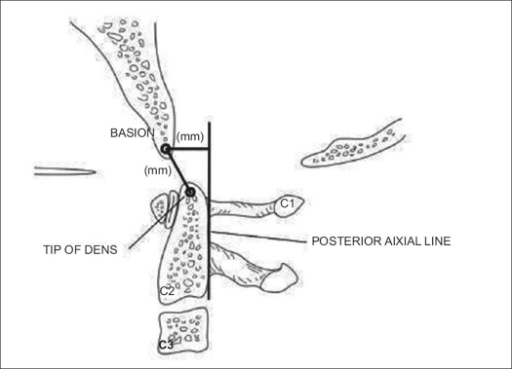
\includegraphics[width=8cm]{BDI.png}
\end{figure}
Definiert als Länge der kürzesten Distanz zwischen dem Mittelpunkt des Ophistons und der Spitze des Denz in Millimetern.


\subsection{Statistik}
\paragraph{Normalbevölkerung}
\paragraph{Traumapatienten}
\paragraph{Validität}
\paragraph{Reliabiliät}

\subsection{Patholgischer Wert}
\subsection{Anwendbarkeit}




\bibliography{../literatur}
\bibliographystyle{dinat}
\end{document}
